\documentclass[12pt]{article}
\usepackage[portuguese]{babel}
\usepackage{natbib}
\usepackage[export]{adjustbox}
\usepackage{float}
\usepackage{url}
\usepackage[utf8x]{inputenc}
\usepackage{mathtools}  
\usepackage{graphicx}
\graphicspath{images}
\usepackage{listings}
\usepackage[margin=2cm]{geometry}
\usepackage{wrapfig}
\renewcommand*{\thesubsubsection}{\alph{subsubsection}.}
\usepackage{multicol}
\usepackage{caption}
\usepackage{xspace}
\usepackage{hyperref}

\begin{document}

\begin{titlepage}

\center % Center everything on the page

\newcommand{\HRule}{\rule{\linewidth}{0.4mm}} % Barra horizontal

\textsc{\LARGE Universidade do Minho}\\[0.5cm]  % Name of your university/college

\vspace{1cm}
\textsc{\large Licenciatura em Engenharia Informática}\\[1.5cm] % Nome do curso
\vspace{0.5cm}

\HRule \\[0.5cm]
{ \LARGE \bfseries } Redes de Computadores \\[0.5cm] % Título
{ \LARGE \bfseries } \textbf{Grupo 135} \\[0.5cm] % Grupo
\HRule \\[1cm]
\vspace{0.1cm}
 
\paragraph{}
\paragraph{}
\textsc{\Large \textbf{TP4: Redes Sem Fios (\textit{Wi-Fi})}}\\[0.75cm] % Nome da UC
\vspace{2.5cm} % Autores
Joana Alves (A93290) \\ \vspace{3mm}
João Machado (A89510) \\ \vspace{3mm} 
Rui Armada (A90468) \\ \vspace{3mm}

\vspace{3cm}


\vspace*{\fill}

{\large Maio 2022}\\[2cm] % Data

\vfill % Fill the rest of the page with whitespace
\end{titlepage}








% ---------- QUESTÕES ---------



\section{Questão 4}

\subsubsection{Observe o conteúdo da tabela ARP. Diga o que significa cada uma das colunas.}

    \begin{figure}[H]
    \centering
    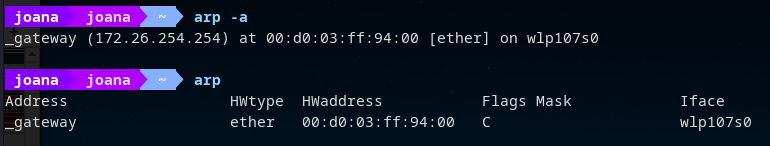
\includegraphics[width=350pt]{prints/Questao4/questao4-ArpTABLE.png}
    \caption{Tabela ARP.} \label{questao4-ARPRequest1}
    \end{figure}
    
    \par Uma tabela ARP é um método de armazenamento de informações descobertas através do protocolo ARP. É usada para registar os pares correspondentes de endereços MAC e endereços IP de dispositivos conectados a uma rede. Cada dispositivo conectado possui a sua própria tabela ARP, que, tal como referido acima, é responsável por armazenar os pares de endereços com os quais um determinado dispositivo já comunicou. Assim, apresentamos uma descrição das várias colunas presentes na tabela ARP.
    
    \begin{center}
        \begin{tabular}{|c|c|}
        \hline
            \cline{1-2}
            Coluna & Descrição  \\
            \hline \hline
            Address & endereço IP destino na rede\\
            HWtype & tipo de \textit{hardware} \\
            HWaddress & endereço MAC do \textit{hardware}\\
            Flags* & informação sobre a entrada \\
            Mask & máscara a aplicar ao endereço IP \\
            Iface & interface de saída \\
            \cline{1-2}
        \end{tabular}
    \end{center}
    
    \par \textbf{*} Neste caso, o valor da coluna é 'C'. Este tipo de entrada é visto quando as entradas são dinamicamente aprendidas pelo protocolo ARP.


    
    





\subsubsection{Qual é o valor hexadecimal dos endereços origem e destino na trama Ethernet que contém a mensagem com o pedido ARP (ARP Request)? Como interpreta e justifica o endereço destino usado?}

    \begin{figure}[H]
    \centering
    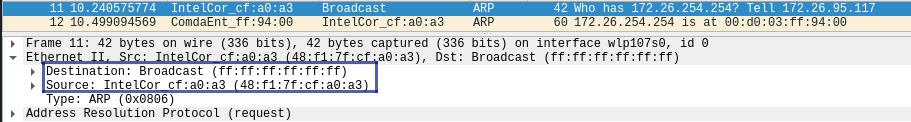
\includegraphics[width=500pt]{prints/Questao4/questao4-firstARP.png}
    \caption{Captura da Trama \textit{Ethernet} com pedido ARP.} \label{questao4-ARPRequest2}
    \end{figure}
    
    \begin{multicols}{2}
    \begin{itemize}
        \item MAC Origem: \textbf{48:f1:7f:cf:a0:a3}  
        \item MAC Destino: \textbf{ff:ff:ff:ff:ff:ff}
    \end{itemize}
    \end{multicols}


    \par A utilização do endereço MAC destino com o valor dos \textit{bits} todos a 1, é uma particularidade do protocolo ARP, isto é, como apagamos a \textit{cache} da tabela ARP, esta não tem qualquer informação de tradução e correspondência entre endereços IP e endereços MAC. Assim, quando, como neste caso, queremos enviar algum pacote para outro dispositivo, temos de primeiro descobrir o seu endereço MAC. Este problema é solucionado colocando o endereço MAC destino com todos os \textit{bits} a 1, representando uma mensagem em \textbf{\textit{broadcast}} (contendo o endereço IP do dispositivo alvo). 
    \par O modo de funcionamento pode ser caracterizado como uma difusão do pedido de \textit{broadcast} do nosso dispositivo por todos os nodos da mesma rede local até encontrar o aparelho que contém o mesmo endereço IP que o endereço IP destino do pedido. De seguida, o aparelho destino (alvo) envia uma resposta (ARP \textit{reply}) à nossa máquina contendo o seu endereço MAC.



\subsubsection{Qual o valor hexadecimal do campo tipo da trama Ethernet? O que indica?}

    \par O valor do campo \textit{type} do cabeçalho da trama \textit{Ethernet} é \textbf{0x0806} que indica que o protocolo encapsulado pela trama é o protocolo ARP.




\subsubsection{Como pode confirmar que se trata efetivamente de um pedido ARP? Identifique que tipo de endereços estão contidos na mensagem ARP? Que conclui?}

    \begin{figure}[H]
    \centering
    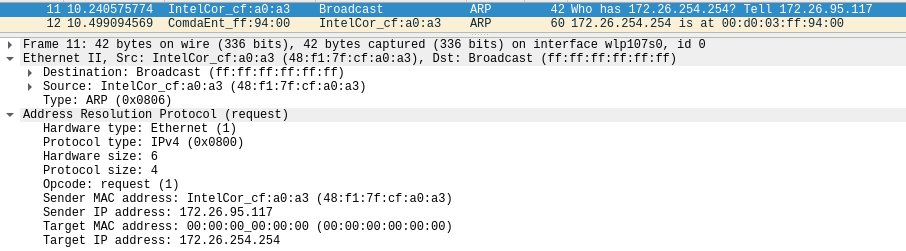
\includegraphics[width=500pt]{prints/Questao4/questao4-firstARP.png.png}
    \caption{Conteúdo ARP.} \label{questao4-ARPRequest-Extended}
    \end{figure}
    
    \paragraph{}
    \par Podemos confirmar que se trata de um pedido ARP pela análise do conteúdo da mensagem ARP, nomeadamente no valor do campo \textit{\textbf{Opcode}}. Este campo indica que tipo de mensagem ARP estamos a tratar, tendo, neste caso, o valor 1 que corresponde a um \textit{\textbf{request}}.
    
    \par Os endereços contidos na mensagem ARP são endereços MAC e IP dos sistemas de origem e destino, ou seja, para cada sistema está indicado o seu endereço IP e correspondente endereço MAC. No entanto, como podemos ver pela Figura \ref{questao4-ARPRequest-Extended}, esta possui o valor do endereço MAC destino (\textit{Target MAC Address}) a zeros. Isto acontece porque, como referido anteriormente, o endereço MAC destino é uma incógnita, sendo, exatamente, o que o protocolo  ARP está a tentar resolver.




\subsubsection{Explicite que tipo de pedido ou pergunta é feita pelo host de origem.}

    \par O \textit{host} de origem envia um pedido (ARP \textit{request}) a todos os nodos presentes na mesma LAN com o objetivo de obter uma resposta (ARP \textit{reply}) do sistema cujo endereço IP corresponde ao endereço IP destino presente na mensagem enviada, contendo esta, também, o endereço MAC do sistema alvo.


\subsubsection{Localize a mensagem ARP que é a resposta ao pedido ARP efetuado. (1) Qual o valor do campo ARP \textit{opcode}? O que especifica? (2) Em que campo da mensagem ARP está a resposta ao pedido ARP? }

    \begin{figure}[H]
    \centering
    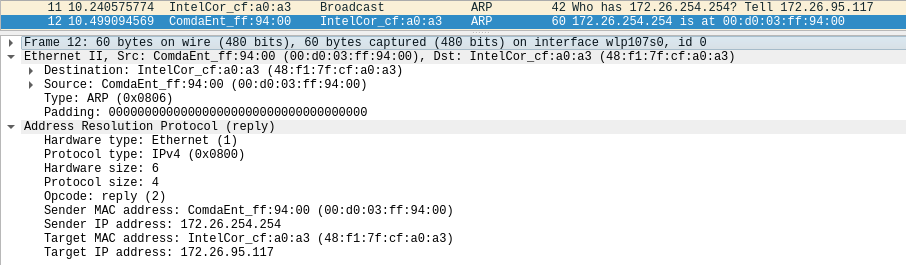
\includegraphics[width=500pt]{prints/Questao4/questao4-responseARP.png}
    \caption{Captura da Trama \textit{Ethernet} com resposta ARP.} \label{questao3-ARPResponse}
    \end{figure}
    
    \
    \par \textbf{(1)} O valor do campo \textit{Opcode} é 2 que corresponde a uma mensagem do tipo \textit{\textbf{ARP reply}}, ou seja, é uma mensagem de resposta a um pedido (\textit{request}) ARP.
    
    \par \textbf{(2)} O conteúdo da resposta ao pedido ARP está presente no campo \textbf{\textit{Sender MAC Address}}, onde podemos denotar a introdução de um endereço MAC válido, contrariamente ao presente no campo \textit{Target MAC Address} do ARP \textit{request} analisado anteriormente.




\newpage
\subsubsection{Na situação em que efetua um ping a outro host, assuma que este está diretamente ligado ao mesmo router, mas noutra subrede, e que todas as tabelas ARP se encontram inicialmente vazias. Esboce um diagrama em que indique claramente, e de forma cronológica, todas as mensagens ARP e ICMP trocadas, até à recepção da resposta ICMP do host destino.}


    \begin{figure}[H]
    \centering
    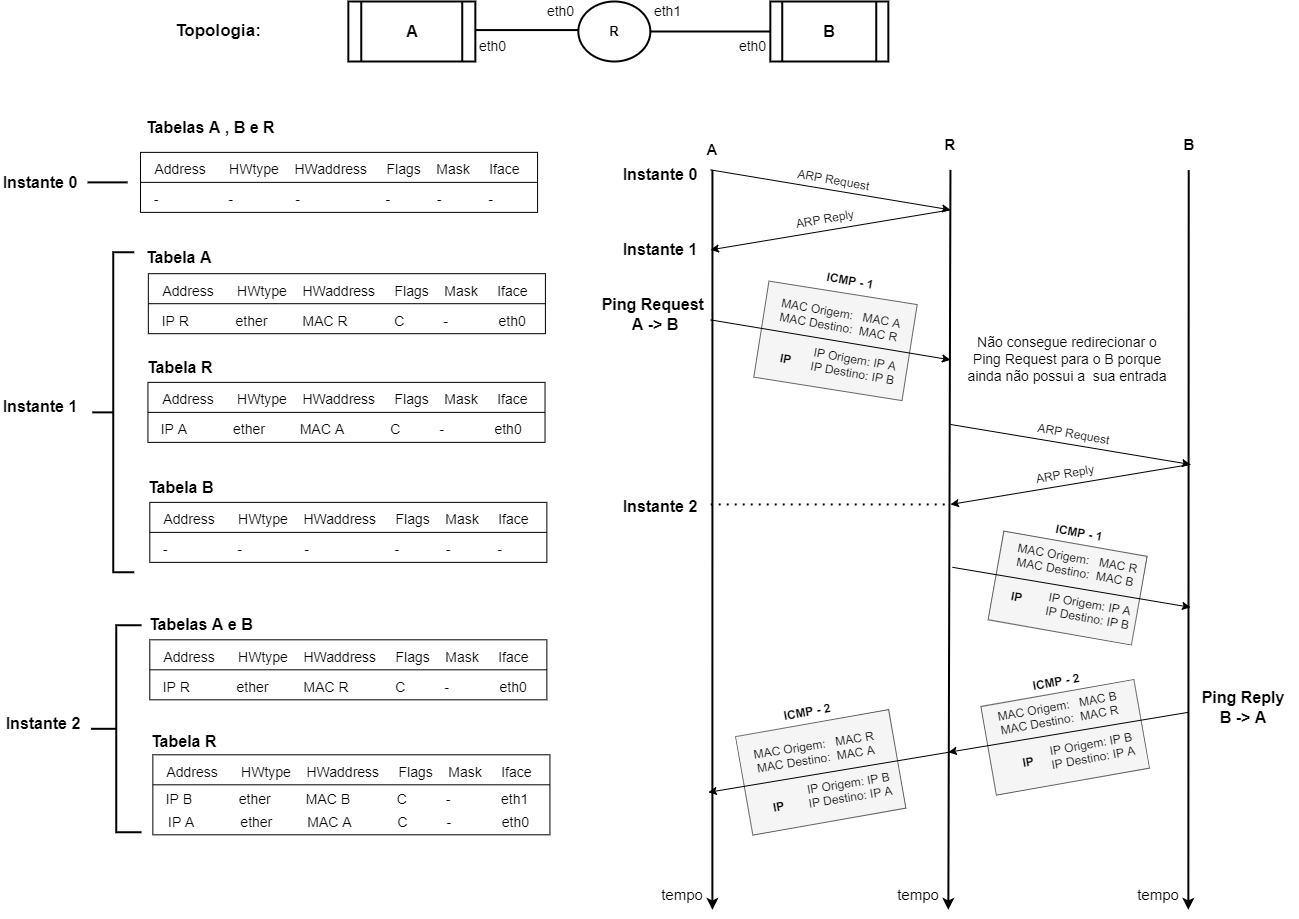
\includegraphics[width=\linewidth]{prints/Questao5/diagramaNOVO.png}
    \end{figure}


\section{Questão 5}

\subsubsection{Através da opção tcpdump verifique e compare como flui o tráfego nas diversas interfaces do dispositivo de interligação no departamento A (LAN partilhada) e no departamento B (LAN comutada) quando se gera tráfego intra-departamento (por exemplo, fazendo ping IPaddr da Bela para Monstro, da Jasmine para o Alladin, etc.) Que conclui?}

    \begin{figure}[H]
    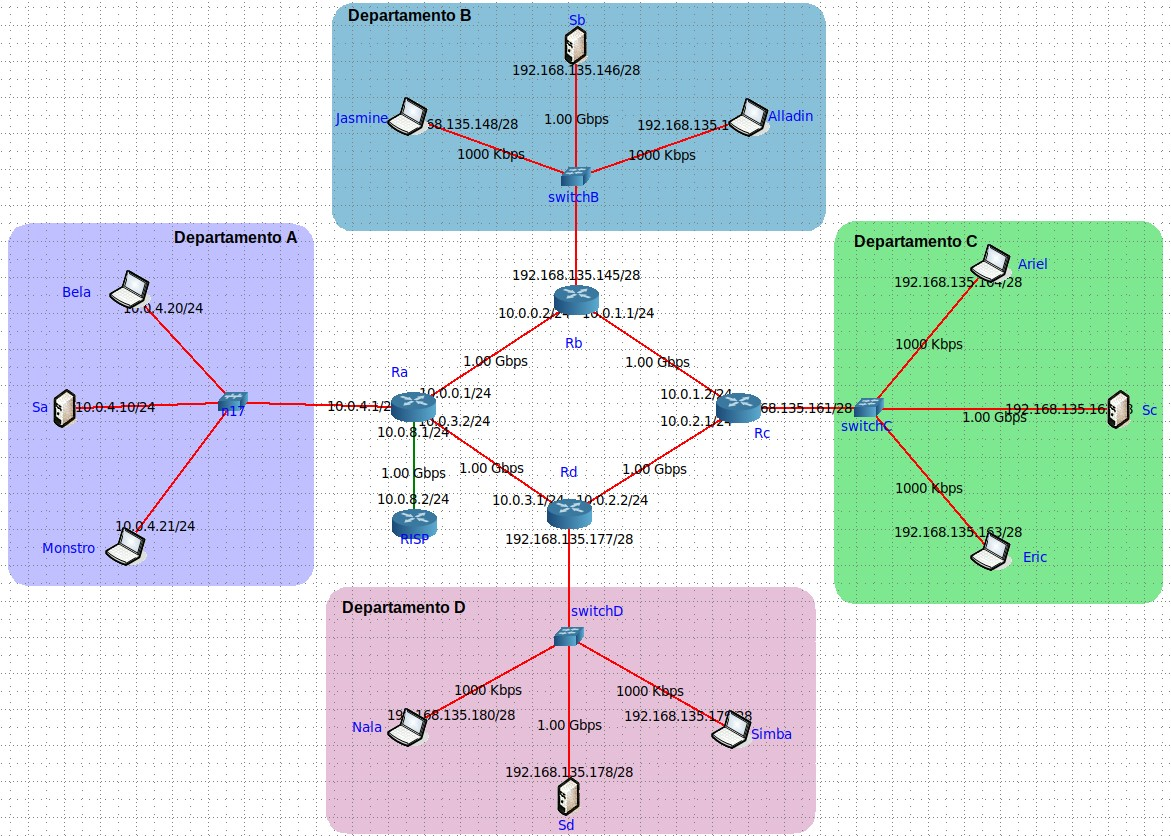
\includegraphics[width=\linewidth]{prints/Questao5/topologia.jpg}
    \caption{Topologia com o \textit{hub} adicionado.} 
    \label{questao5-topologia}
    \end{figure}
    

    \par Como podemos ver pela Figura \ref{questao5-topologia}, os endereços IP dos dispositivos Bela, Monstro e servidor Sa foram alterados em consequência da inserção do \textit{hub} e remoção do \textit{switch}. No entanto, o grupo optou por não voltar a alterar os endereços para os obtidos com o exercício de \textit{subnetting} do trabalho prático anterior, uma vez que não não iria alterar o comportamento esperado neste exercício em particular. Os testes foram realizados da seguinte forma: executou-se um \textit{ping} de um \textit{host} A para outro \textit{host} B e executou-se o comando \textit{tcpdump} num \textit{host} C não envolvido na comunicação do \textit{ping}. Assim, no \textbf{departamento A} executamos o comando \textit{ping} do \textit{host} Monstro para Bela e o comando \textit{tcpdump} no servidor Sa. No caso do \textbf{departamento B}, executamos o comando \textit{ping} do \textit{host} Alladin para Jasmine e o comando \textit{tcpdump} no servidor Sb. Por fim, obtivemos os seguintes resultados com os vários comandos:
            
            
    \begin{minipage}{0.5\linewidth}
        \centering
            \begin{figure}[H]
            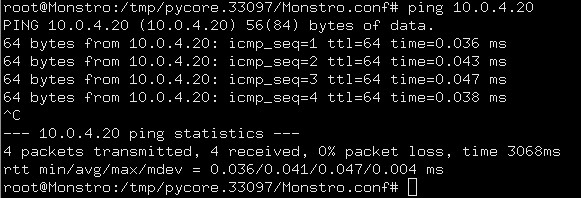
\includegraphics[width=\linewidth]{prints/Questao5/A-Monstro-Bela.jpg}
            \caption{Ping do \textit{host} Monstro para Bela.} \label{questao5-ping-A}
            \end{figure}
    \end{minipage}
    \begin{minipage}{0.5\linewidth}
        \centering
            \begin{figure}[H]
            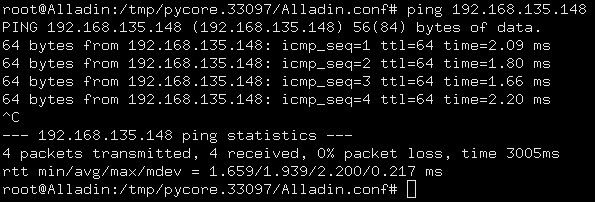
\includegraphics[width=\linewidth]{prints/Questao5/B-Alladin-Jasmine.jpg}
            \caption{Ping do \textit{host} Alladin para Jasmine.} \label{questao5-ping-B}
            \end{figure}
    \end{minipage}

    \paragraph{}
    \paragraph{}
    \begin{figure}[H]
    \centering
    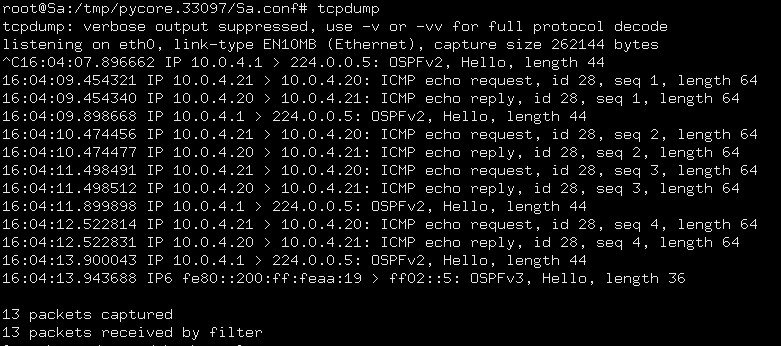
\includegraphics[width=400pt]{prints/Questao5/A-Sa.jpg}
    \caption{Comando \textit{tcpdump} no servidor Sa (LAN partilhada).} \label{questao5-tcpdump-A}
    \end{figure}
    
    \begin{figure}[H]
    \centering
    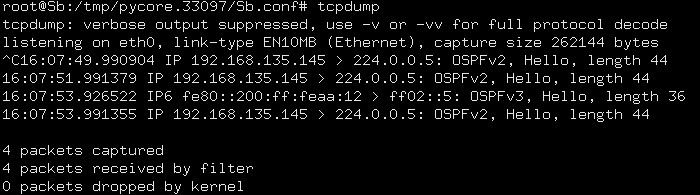
\includegraphics[width=400pt]{prints/Questao5/B-Sb.jpg}
    \caption{Comando \textit{tcpdump} no servidor Sb (LAN comutada).} \label{questao5-tcpdump-B}
    \end{figure}
    
    
    
    \par Existem várias diferenças entre \textit{hubs} e \textit{switches}, sendo a mais distinta a camada protocolar onde operam, isto é, o \textit{hub} opera ao nível físico enquanto que os \textit{switches} operam na camada de ligação lógica.
    Para além disto, os \textit{\textbf{hubs}} são dispositivos que repetem o sinal que chega através de uma porta de entrada para todas as outras portas, isto é, difundem o sinal por todas as interfaces que possuem.
    No que toca aos \textit{\textbf{switches}}, estes, com a ajuda de uma tabela de \textit{switching} (comutação), comutam as tramas para a interface de saída apropriada. No entanto, caso se depare com uma trama que não tem um endereço que conste na tabela, este difunde a trama por todas as suas interfaces, obtendo, neste caso em específico, um comportamento semelhante ao \textit{hub}.

    \par Assim, e tendo estas distinções em mente, conseguimos de imediato notar diferenças no resultado do comando \textit{tcpdump} nas duas situações. Na \textbf{LAN partilhada}, o terceiro \textit{host} não envolvido diretamente na comunicação também recebeu os pacotes, provando assim a particularidade dos \textit{hubs} no que toca à difusão das comunicações por todas as portas dos mesmos.
    No caso da \textbf{LAN comutada}, denotamos que o resultado da captura é vazio no que toca a pacotes relacionados com a comunicação derivada do comando \textit{ping}, provando assim a diferença de comportamento do \textit{switch} com o \textit{hub}, pois o tráfego é comutado para as interfaces devidas, não sendo difundido pela rede.




%\newpage
\subsubsection{Construa manualmente a tabela de comutação do switch do Departamento B, atribuindo números de porta à sua escolha.}

    \paragraph{}
    \par Para obtermos os endereços MAC dos vários sistemas diretamente ligados ao \textit{switch}, executamos o comando \textit{\textbf{ifconfig -a}}. Assim, obtivemos os seguintes endereços, notando que no \textit{router} o endereço da interface \textit{eth2} corresponde à interface de ligação ao \textit{switch}.

    \begin{minipage}{0.5\linewidth}
        \centering
            \begin{figure}[H]
            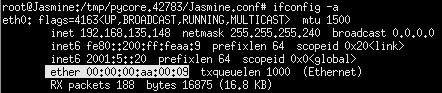
\includegraphics[width=\linewidth]{prints/Questao5/Jasmine.jpg}
            \caption{Endereço MAC Jasmine.} \label{questao5-MAC-Jasmine}
            \end{figure}
    \end{minipage}
    \begin{minipage}{0.5\linewidth}
        \centering
            \begin{figure}[H]
            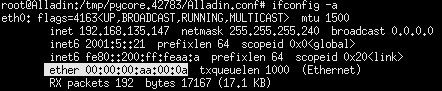
\includegraphics[width=\linewidth]{prints/Questao5/Alladin.jpg}
            \caption{Endereço MAC Alladin.} \label{questao5-MAC-Alladin}
            \end{figure}
    \end{minipage}
    
    \begin{minipage}{0.5\linewidth}
        \centering
            \begin{figure}[H]
            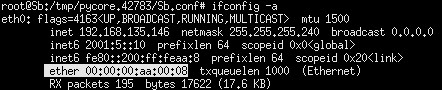
\includegraphics[width=\linewidth]{prints/Questao5/Servidor.jpg}
            \caption{Endereço MAC Servidor.} \label{questao5-MAC-Servidor}
            \end{figure}
    \end{minipage}
    \begin{minipage}{0.5\linewidth}
        \centering
            \begin{figure}[H]
            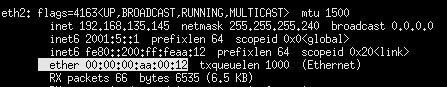
\includegraphics[width=\linewidth]{prints/Questao5/Router.jpg}
            \caption{Endereço MAC Alladin.} \label{questao5-MAC-Router}
            \end{figure}
    \end{minipage}
    
    \paragraph{}
    \par Após obtermos os endereços MAC, desenvolvemos um esboço da topologia da subrede do Departamento B (incluindo o \textit{router}) para assim termos uma visão simplificada dos sistemas integrantes. Como tal, obtivemos a seguinte tabela de comutação:
    
    \begin{figure}[H]
    \centering
    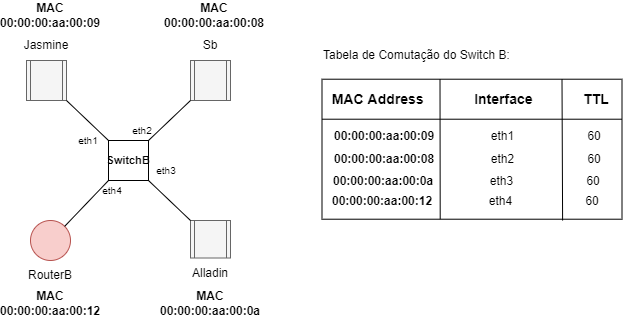
\includegraphics[width=450pt]{prints/Questao5/switch.png}
    \label{questao5-switchTable}
    \end{figure}


\section{Questão 6}



\subsubsection{Identifique uma sequência de tramas que corresponda a um processo de associação completo entre a STA e o AP, incluindo a fase de autenticação.}

    \par Um processo de associação completo envolve vários tipos de tramas como: \textit{Association Request}, \textit{Association Response}, \textit{Authentication} e, por fim, \textit{Acknowledgement}. Assim, desenvolvemos um filtro que pesquisasse todas estas tramas para facilitar a pesquisa de todo o processo. Os valores dos subtipos no filtro foram utilizados de acordo com o anexo fornecido dos docentes. Apresentamos, então, o filtro desenvolvido seguido do processo de associação identificado:
    
    \vspace{10pt}
    \begin{minipage}{\linewidth}
        \centering
        \fbox{
        \parbox{250pt}{
		    (wlan.fc.type\_subtype $==$ 0x00) \textbf{or} (wlan.fc.type\_subtype $==$ 0x01)
		    \textbf{or} (wlan.fc.type\_subtype $==$ 0x0b) \textbf{or} (wlan.fc.type\_subtype  \hspace{22pt}$==$\hspace{22pt} 0x1d) 
        }
    }
    \end{minipage}

    \begin{figure}[H]
        \centering
        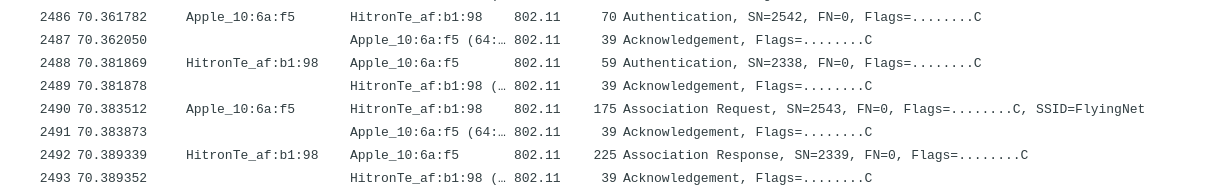
\includegraphics[width=500pt]{Prints/Questao6/rc1.png}
        \caption{Processo de associação completo entre a STA e o AP} \label{questao6-1}
    \end{figure}








\subsubsection{Efetue um diagrama que ilustre a sequência de todas as tramas trocadas no processo.}

    \par A partir das tramas obtidas na alínea anterior, desenvolvemos o seguinte diagrama ilustrando as mensagens trocadas entre STA e o AP durante o processo de associação:

    \begin{figure}[H]
        \centering
        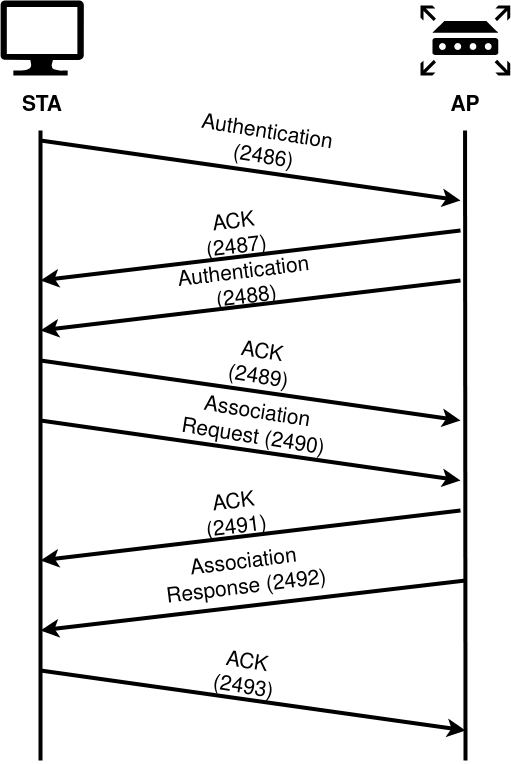
\includegraphics[width=150pt]{Prints/Questao6/STA-AP.png}
        \caption{Sequência de tramas trocadas durante o processo} \label{questao6-2}
    \end{figure}


\section{Questão 7}


\subsubsection{Considere a trama de dados nº431. Sabendo que o campo \textit{Frame Control} contido no cabeçalho das tramas 802.11 permite especificar a direccionalidade das tramas, o que pode concluir face à direccionalidade dessa trama, será local à WLAN?}

    \par Ao analisarmos a trama, mais especificamente o campo \textit{Frame Control}, conseguimos denotar o valor das \textit{flags} do mesmo. Para a pergunta em questão, a \textit{flag} que procuramos é a \textbf{DS \textit{status}}, tendo esta dois valores a preencher: \textit{To} DS/AP (destino no AP) e \textit{From} DS/AP (origem no AP). De acordo com a trama, os valores de \textit{To} DS e \textit{From} DS são, respetivamente, \textbf{0} e \textbf{1}, ou seja, estamos perante uma trama que foi enviada através de um AP para um STA, podendo concluir que a trama é local à WLAN.

    \begin{figure}[H]
    \centering
    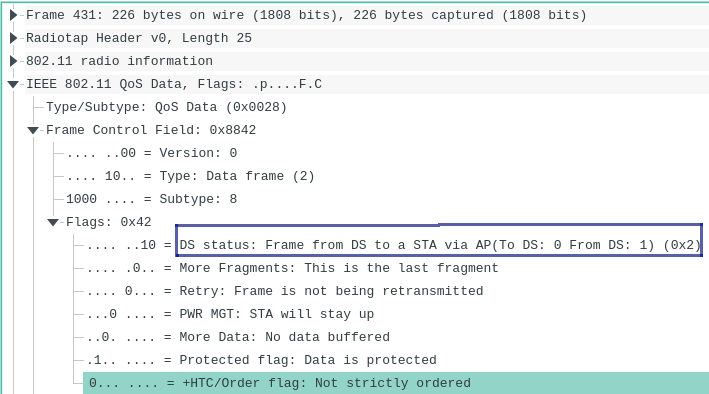
\includegraphics[width=400pt]{Prints/Questao7/questao7-A.png}
    \caption{Captura da Trama Nº 431.} \label{questao7-1-trama431}
    \end{figure}





\vspace{20pt}
\subsubsection{Para a trama de dados nº431, transcreva os endereços MAC em uso, identificando qual o endereço MAC correspondente ao host sem fios (STA), ao AP e ao \textit{router} de acesso ao sistema de distribuição?}

    \par Para além da análise da trama, utilizamos a funcionalidade \textit{hexdump} do \textit{Wireshark}, tendo assim acesso aos \textit{bytes} ordenados da trama. Como tal, conseguimos distinguir três endereços: \textit{receiver} (\textbf{64:9a:be:10:6a:f5}), \textit{transmitter} (\textbf{bc:14:01:af:b1:98}) e \textit{router interface} (\textbf{bc:14:01:af:b1:98}).

    \par Como podemos verificar, o endereço do \textit{host} sem fios (STA) corresponde ao endereço do \textit{receiver}, logo esta trama tem como destino o mesmo. Relativamente aos endereços do AP e do \textit{router}, estes são idênticos, o que nos leva a concluir que o AP realiza tanto as funcionalidades de \textit{routing} como de transmissão de tramas.
    
    \begin{figure}[H]
    \centering
    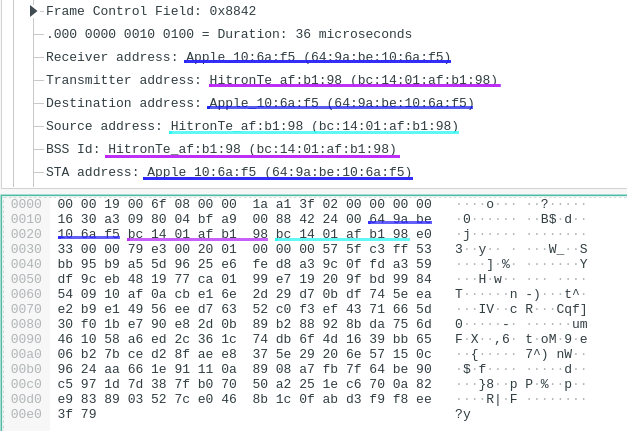
\includegraphics[width=350pt]{Prints/Questao7/questao7-B-1.png}
    \caption{Endereços MAC contidos na trama.} \label{questao7-2-enderecos}
    \end{figure}




    





\subsubsection{Como interpreta a trama nº433 face à sua direcionalidade e endereçamento MAC?}

    \begin{figure}[H]
    \centering
    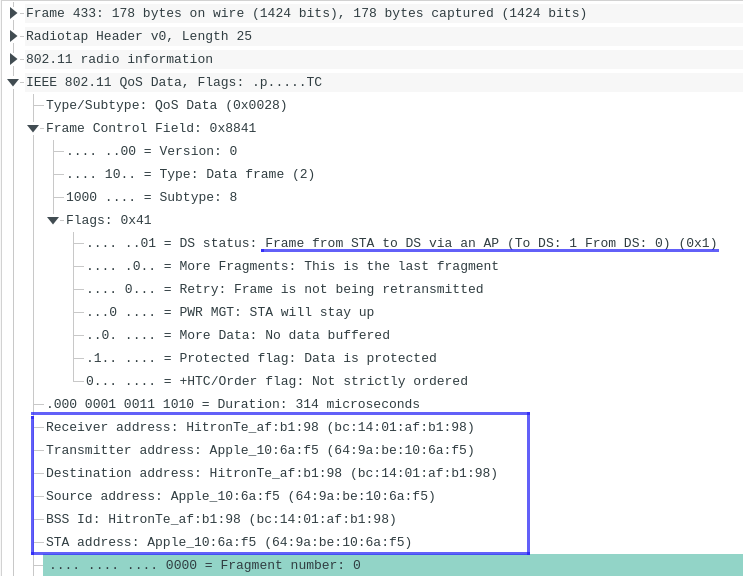
\includegraphics[width=300pt]{Prints/Questao7/questao7-433.png}
    \caption{Captura da Trama Nº 433.} \label{questao7-1-trama433}
    \end{figure}

    \par Ao analisarmos as \textit{flags} presentes no campo \textit{Frame Control}, denotamos que os valores de \textit{To} DS e \textit{From DS} são, respetivamente, 1 e 0, ou seja, contrariamente à trama analisada anteriormente, esta é direcionada ao AP tendo como origem o STA. Para além disto, poderíamos chegar à mesma conclusão a partir da análise dos endereços MAC presentes na trama: \textit{receiver} ((\textbf{bc:14:01:af:b1:98})), \textit{transmitter} (\textbf{64:9a:be:10:6a:f5}) e \textit{destination} (\textbf{bc:14:01:af:b1:98}).







\subsubsection{Que subtipo de tramas de controlo são transmitidas ao longo da transferência de dados acima mencionada? Tente explicar porque razão têm de existir (contrariamente ao que acontece numa rede Ethernet.)}

    \par Ao longo de uma transferência de dados são transmitidas tramas de controlo do subtipo \textit{Request To Send} e \textit{Clear To Send}. Estas tramas têm como objetivo evitar colisões e controlar a transmissão de dados pelo meio, uma vez que vários dispositivos podem estar ligados a um AP e, caso transmitam simultaneamente, vão existir colisões e como consequência a corrupção de pacotes.
    
    \par Assim, podemos resumir o comportamento destas tramas de controlo da seguinte forma: o STA envia tramas com pedidos de conexão (RTS) para o AP, respondendo o AP, em \textit{broadcast}, uma trama CTS. A trama CTS é "ouvida"\xspace por todos os nós, permitindo ao STA enviar os dados ao AP sem interrupções.

    \par Contrariamente, nas redes \textit{Ethernet}, este sistema não é implementado, pois estas utilizam dispositivos como \textit{switches} e \textit{hubs} que conseguem redirecionar e distribuir o tráfego na rede, em particular, na utilização de \textit{switches}, cada dispositivo tem um canal de transmissão único e direto, permitindo assim evitar colisões.





\vspace{10pt}
\subsubsection{O uso de tramas \textit{Request To Send} e \textit{Clear To Send}, apesar de opcional, é comum para efetuar "pré-reserva" do acesso ao meio quando se pretende enviar tramas de dados, com o intuito de reduzir o número de colisões resultante maioritariamente de STAs escondidas. Para o exemplo acima, verifique se está a ser usada a opção RTS/CTS na troca de dados entre a STA e o AP/Router da WLAN, identificando a direccionalidade das tramas e os sistemas envolvidos. Dê um exemplo de uma transferência de dados em que é usada a opção RTC/CTS e um outro em que não é usada}

    \par Para verificarmos se existiu algum controlo de colisões através das tramas RTS e CTS, começamos por analisar as tramas capturadas nos instantes imediatamente antes e depois da trama nº 433. Desta forma, obtivemos as seguintes tramas, não obtendo quaisquer tramas de controlo de colisões:
    
    \begin{figure}[H]
    \centering
    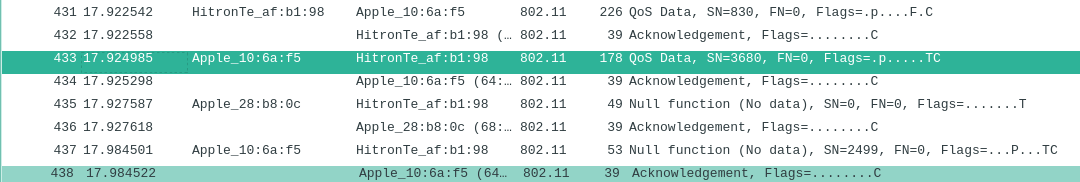
\includegraphics[width=500pt]{Prints/Questao7/questao7-Ultima.png}
    \caption{Tramas capturadas na envolvência da trama nº433.} \label{questao7-redor}
    \end{figure}
    
    \par Assim, para encontrarmos uma transferência de dados que utilize este controlo e de modo a facilitar a sua pesquisa no ficheiro de captura, desenvolvemos o seguinte filtro que irá filtrar todas as tramas RTS e CTS assim como todas as tramas de dados, tendo retirado, novamente, os valores dos subtipos do anexo dos docentes.
    
    \vspace{20pt}
    \begin{minipage}{\linewidth}
        \centering
        \fbox{
        \parbox{390pt}{
		    (wlan.fc.type\_subtype $==$ 0x1b) \textbf{or} (wlan.fc.type\_subtype $==$ 0x1c)
		    \textbf{or} 
		    \par
		    (wlan.fc.type\_subtype $>$= 0x20 \textbf{and} wlan.fc.type\_subtype $<$= 0x2f) 
        }
    }
    \end{minipage}
    
    
    \vspace{10pt}
    \par Após a aplicação do filtro, o \textit{Wireshark} apresentou várias tramas que obedeciam ao mesmo, tendo o grupo captado duas transmissões de dados que diferem na sua direcionalidade, ou seja, uma com a comunicação no sentido AP -$>$ STA e outra no sentido STA -$>$ AP.
    
    \begin{figure}[H]
    \centering
    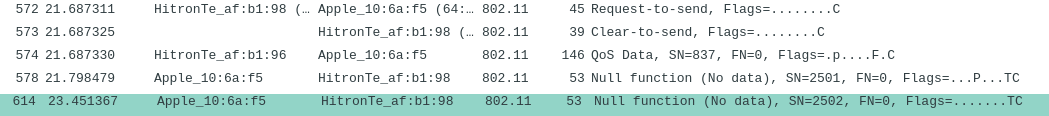
\includegraphics[width=500pt]{Prints/Questao7/questao7-AP2STA.png}
    \caption{Conjunto de tramas no sentido AP -$>$ STA.} \label{questao7-ap2sta}
    \end{figure}
    
    \begin{figure}[H]
    \centering
    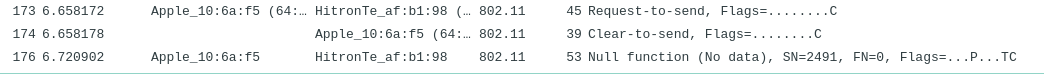
\includegraphics[width=500pt]{Prints/Questao7/questao7-STA2AP.png}
    \caption{Conjunto de tramas no sentido STA -$>$ AP.} \label{questao7-sta2ap}
    \end{figure}
    
    \par Como podemos verificar pelas Figuras \ref{questao7-ap2sta} e \ref{questao7-sta2ap}, o dispositivo de origem envia uma trama RTS ao dispostivo destino e, depois de aceite, através do envio de uma segunda trama (CTS), trocam dados entre si assim como tramas de confirmação (\textit{Acknowledgement}).



\section{Conclusão}
    
    \par Com a conclusão deste guião prático, encontramo-nos, em geral, satisfeitos com o trabalho desenvolvido, tendo alcançado todos os objetivos propostos pelos docentes no enunciado.
    
    \par Em particular, este trabalho prático incidiu sobre a resolução de vários exercícios e problemas da área de redes, nomeadamente as redes sem fios (\textit{Wi-Fi}). Assim, o grupo teve a oportunidade de aprofundar os seus conhecimentos no estudo de endereços MAC, interpretação do protocolo 802.11 e, por fim, utilização de controlo de colisões. Para além disso, mais uma vez, foi necessário o manuseamento da ferramenta \textit{wireshark}, provando, novamente, a sua utilidade prática no contexto de análise de tráfego. 

    \par Em suma, a construção e desenvolvimento deste trabalho prático permitiu a todo o grupo aprofundar os seus conhecimentos no que toca às redes sem fios, atingindo uma ampla percepção de vários assuntos englobados pelas mesmas.

\end{document}